
We experimented with the following levels of carbon tax: \textsterling10, \textsterling20 and \textsterling70 with demand decreasing 1\% per year. We chose this due to the increasing efficiency of homes, industy and technology, and due to the recent trend in the UK. We run each scenario 8 times each to capture the stochastic nature of the process. Via the observation of the emergent investment behaviour until 2050, an understanding of how real life investors may behave emerges.


Figure \ref{fig:demand99carbon10} shows that with a carbon tax of \textsterling10, whilst renewable technology does grow, gas power plants provides the majority of supply in each year. However, at a level of \textsterling20 the increase in wind turbines is enough to match gas turbines. A carbon tax of \textsterling70, however, shows a near 100\% uptake of wind turbines.

It is infeasible for the power supply to be provided solely by wind turbines today. This overestimation, however, is due to the low time granularity of the model \cite{Collins2017}. This scenario therefore assumes perfect storage capabilities.






%\FloatBarrier








%\begin{figure}[h]
%	\begin{center}
%		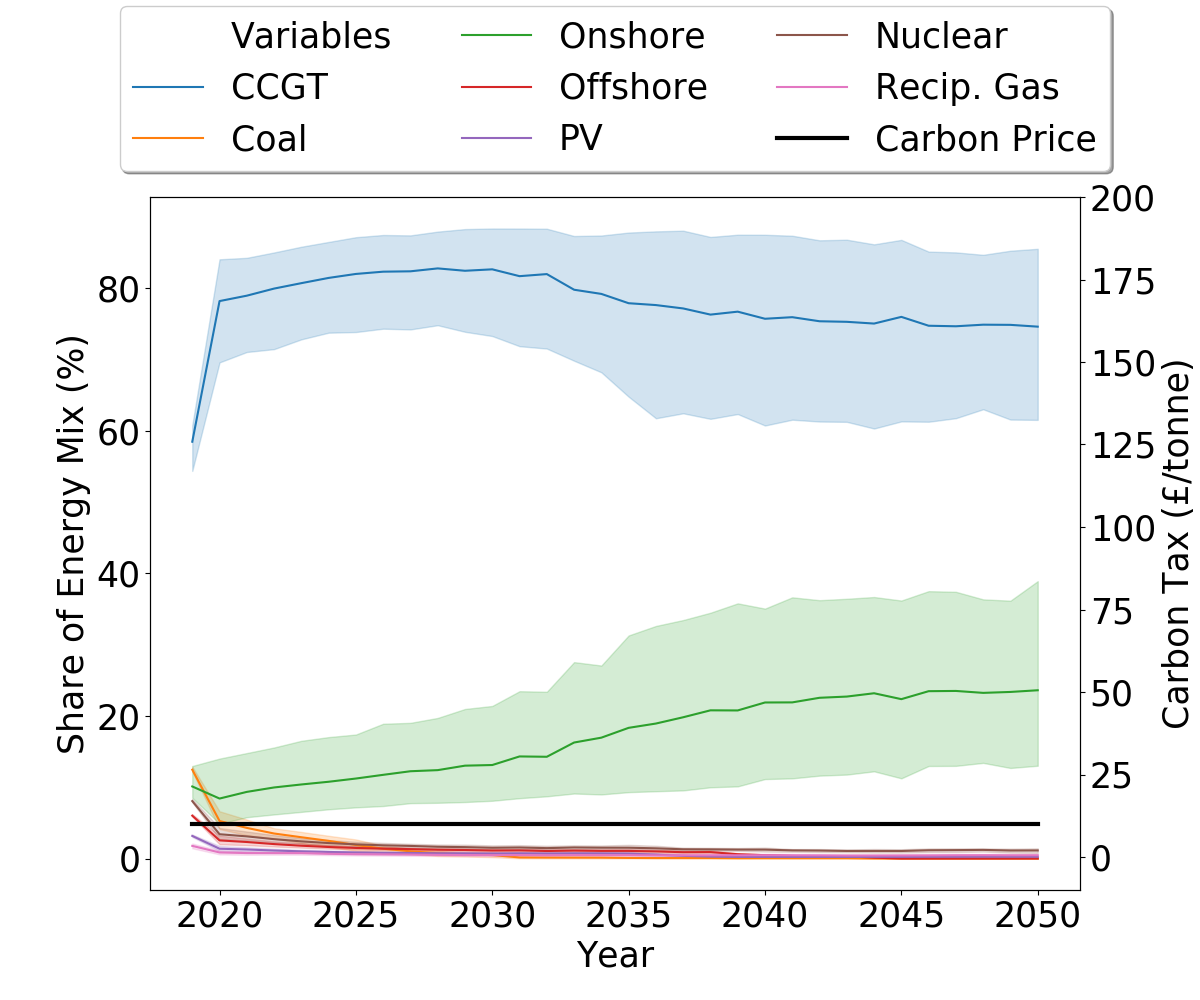
\includegraphics[width=0.5\textwidth]{figures/scenarios/demand099-carbon10-datetime.png}
%		\caption{Demand decreasing by 1\% per year and a carbon tax of \textsterling10}
%		\label{fig:demand99carbon10}
%	\end{center}
%\end{figure}
%
%\begin{figure}[h]
%	\begin{center}
%		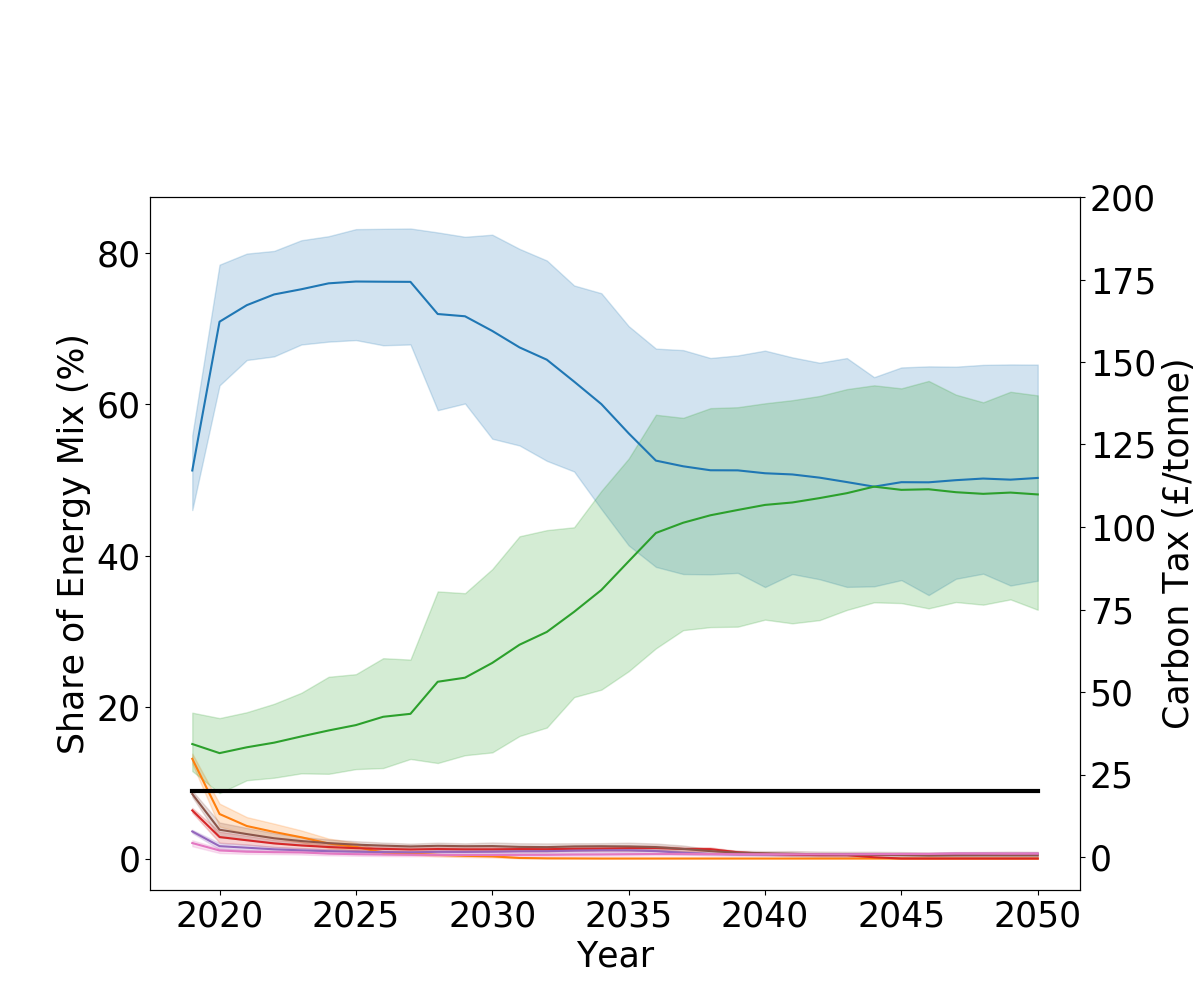
\includegraphics[width=0.5\textwidth]{figures/scenarios/demand099-carbon20-datetime.png}
%		\caption{Demand decreasing by 1\% per year and a carbon tax of \textsterling20}
%		\label{fig:demand99carbon10}
%	\end{center}
%\end{figure}
%
%
%
%\begin{figure}[h]
%	\begin{center}
%		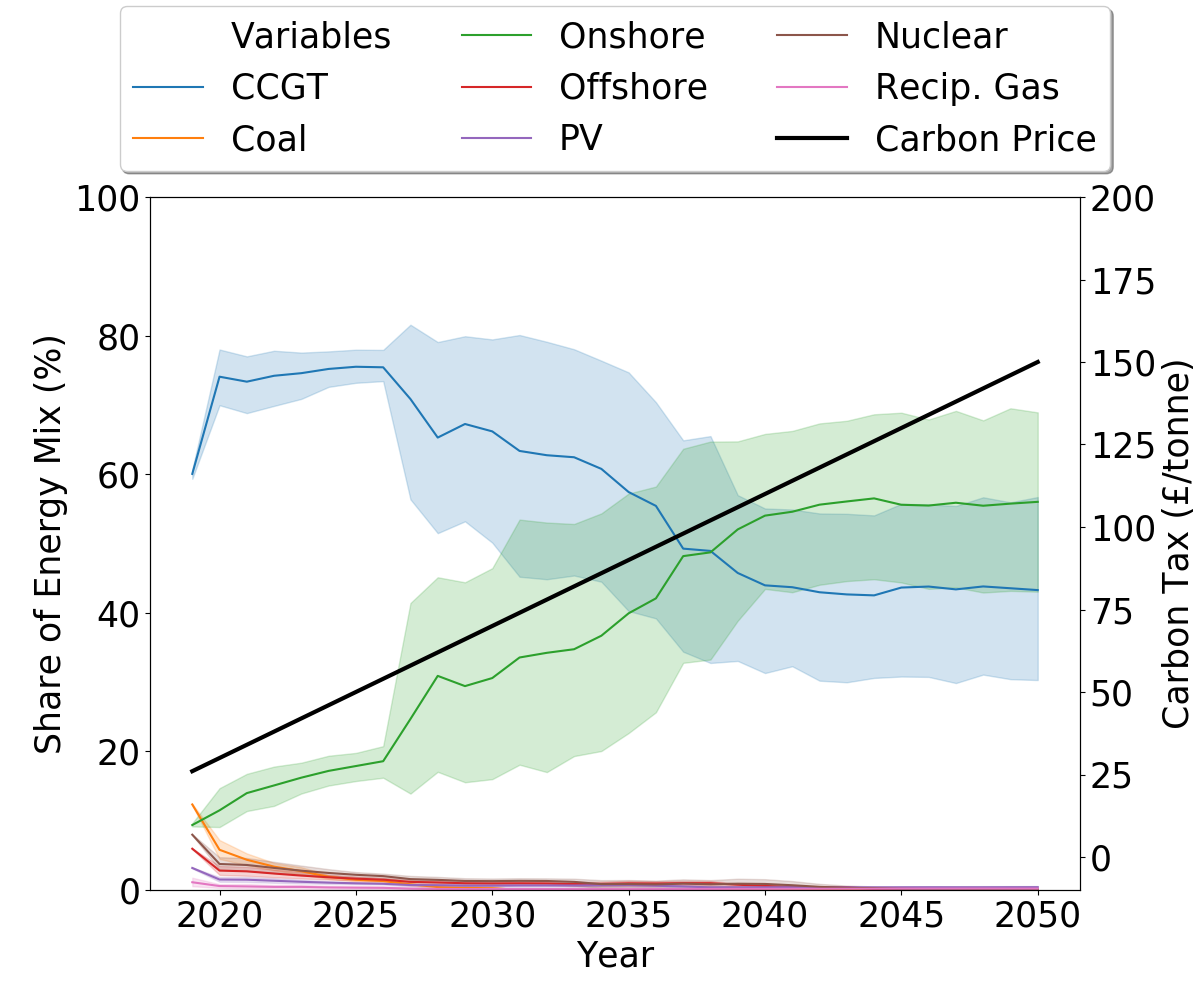
\includegraphics[width=0.5\textwidth]{figures/scenarios/demand099-carbon18-datetime.png}
%		\caption{Demand decreasing by 1\% per year and a carbon tax of \textsterling20}
%		\label{fig:demand99carbon10}
%	\end{center}
%\end{figure}
%
%
%
%\begin{figure}[h]
%	\begin{center}
%		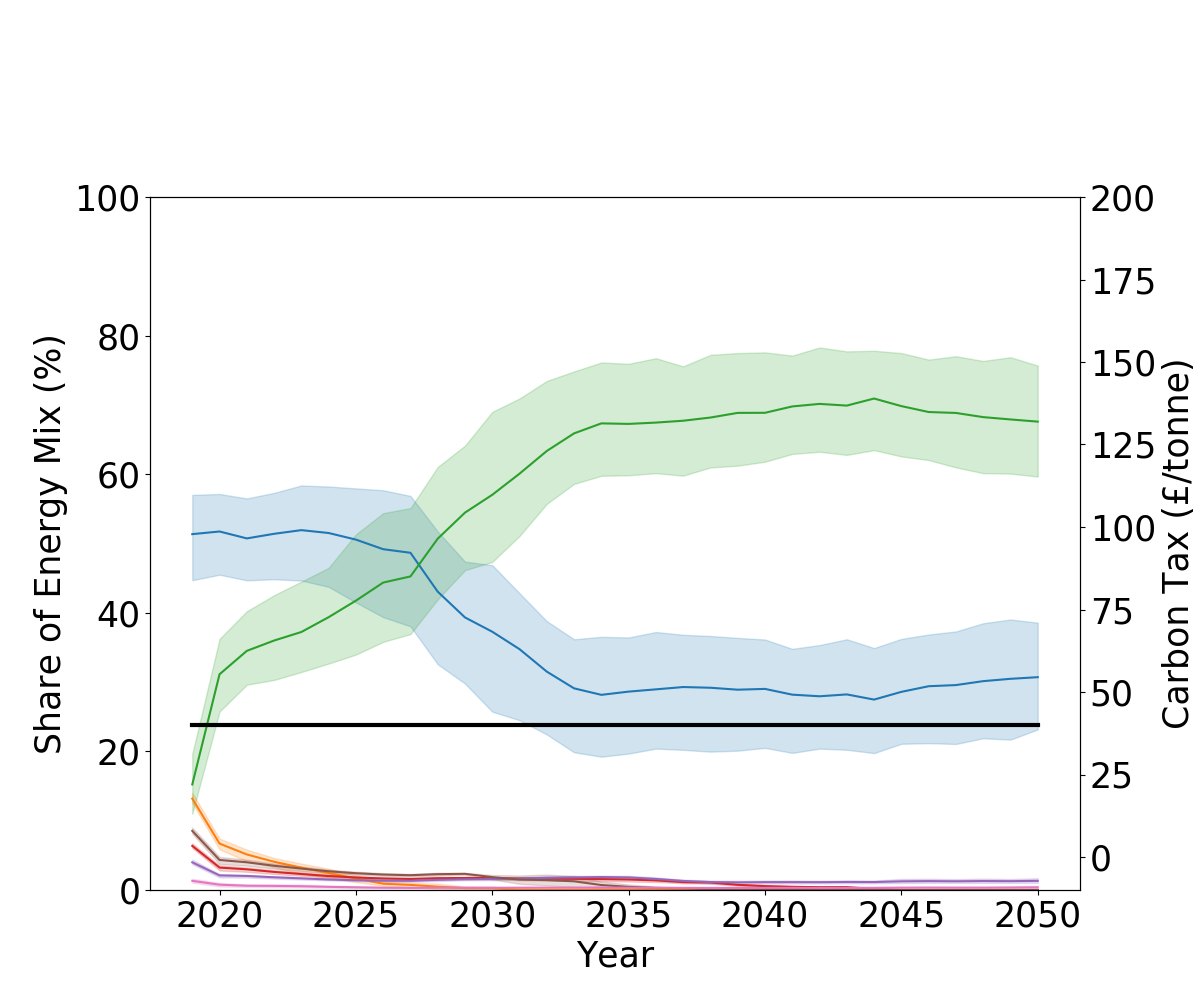
\includegraphics[width=0.5\textwidth]{figures/scenarios/demand099-carbon40-datetime.png}
%		\caption{Demand decreasing by 1\% per year and a carbon tax of \textsterling20}
%		\label{fig:demand99carbon10}
%	\end{center}
%\end{figure}











%\begin{itemize}
%	\item Effect of different carbon tax on investments made.
%	\item Effects of different demand scenarios. (High peaks, high growth, high reduction in demand)
%	\item Effects of high fuel prices.
%	\item Different costs of capital (eg. Borrowing for Nuclear of interest rate to equal 2\% at government bonds rate, as opposed to 10\% for private companies.)
%	\item Different learning rates for renewable costs.
%	\item The effect of long term carbon tax policy (eg. Carbon price known for next 25 years) vs short term changes in carbon tax.
%\end{itemize}
